L'application \textit{symbolist} veut s'abstraire du canevas de la notation traditionnelle, et même de tout autre système d'écriture préétabli, pour proposer aux compositeurs un environnement d'expression graphique libre, proche de l'usage du papier (voir section \ref{sec:geneseSymbolist}).
Cependant, ajouter certains concepts structurants au système de notation de \textit{symbolist} est un réel soutien à la pensée compositionnelle. A cet égard, deux concepts tirés de la CWMN, les concepts de \textit{staff} et de \textit{clef}, ont été intégrés à l'application. 
De plus, dans un souci d'exhaustivité et étant donné les pratiques de notation majoritairement utilisées par les compositeurs de musique contemporaine (voir annexe \ref{sec:analyseBesoins}, page~\pageref{sec:analyseBesoins}), les symboles de la CWMN ont été ajoutés à la palette \textit{symbolist} comme une contribution de ce stage.

\subsection{Concept de staff} 
\label{subsec:conceptDeStaff}
Le concept de \textit{staff} (\gls{portee} en anglais) a été défini et implémenté dans \textit{symbolist}.
Dans notre application, un \textit{staff} peut être représenté graphiquement par n'importe quel symbole qui sera alors considéré comme le symbole référent. Chaque symbole d'une partition \textit{symbolist} possède un message \texttt{/staff} dans le bundle OSC les décrivant. Par exemple, un symbole est attaché au staff d'identifiant 12 si son message \texttt{/staff} vaut 12.
Les symboles de la partition qui sont attachés à un \textit{staff} se voient attribuer une valeur temporelle de départ et de fin correspondant à leur point de départ et de fin vis à vis du symbole référent.
Le staff est une manière d'ordonner horizontalement (localement) les symboles d'une partition \textit{symbolist}. 
La figure \ref{fig:exempleDeStaff} montre un exemple de partition \textit{symbolist} composé d'un \textit{staff}, avec plusieurs symboles attachés, et de symboles libres.

\begin{figure}[H]
	\centering
	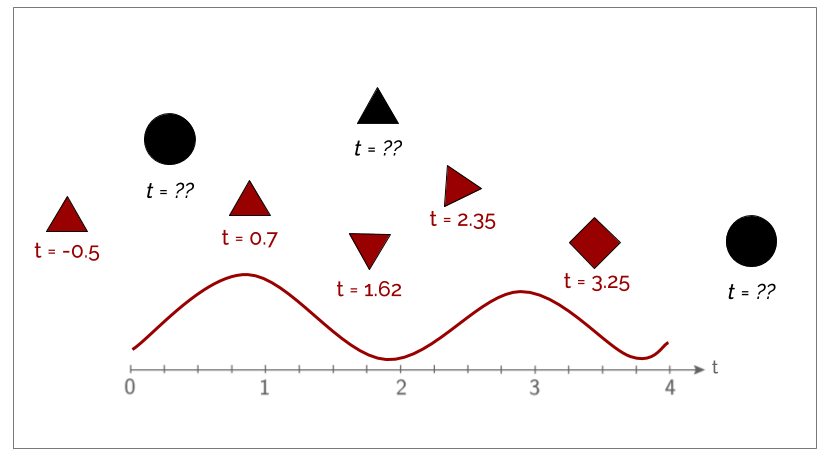
\includegraphics[keepaspectratio=true, width=0.8\textwidth]{ModeleDeNotation/i/staffConcept.png}
	\caption{Définition d'un staff dans une partition symbolist}
	\label{fig:exempleDeStaff}
	\small
	\it
	Le cadre représente une partition \emph{symbolist}. En rouge, le symbole référent du \emph{staff} (la courbe), et les symboles attachés au \emph{staff}. En noir, les symboles libres, sans positionnement temporel.
	Le temps de départ (position de l'extrémité gauche sur l'axe gradué) est donné pour chaque symbole attaché au staff et pour le symbole référent.
\end{figure}

Il est notable, dans la figure \ref{fig:exempleDeStaff}, qu'un symbole attaché à un staff n'est pas contraint de commencer dans l'intervalle temporel du symbole référent. Par exemple, le triangle placé à $t = -0.5$ est en dehors de l'intervalle temporel de la courbe qui commence à $t = 0$.

Comme vu en section \ref{sec:analyseSymbolist}, l'application \textit{symbolist}, dans sa version objet pour \textit{Max} et \textit{OpenMusic}, peut lancer une lecture temporelle de sa partition courante (grâce à l'envoi du message \texttt{time} dans Max, et à la barre de lecture intégrée dans \textit{OpenMusic}). A ce sujet, une lecture temporelle d'une partition \textit{symbolist} n'est possible que lorsqu'au moins un \textit{staff} a été défini. Dans le cas contraire, aucun intervalle temporel n'est présent dans la partition. Lorsque qu'un \textit{staff} a été créé et qu'une lecture temporelle est lancée, une barre de lecture apparaît dans l'interface \textit{symbolist}, accompagné de l'affichage du temps courant. La figure \ref{fig:readingTheScore} donne un exemple de lecture temporelle d'une partition \textit{symbolist}.

\begin{figure}[H]

\centering
\begin{minipage}{0.45\textwidth}
	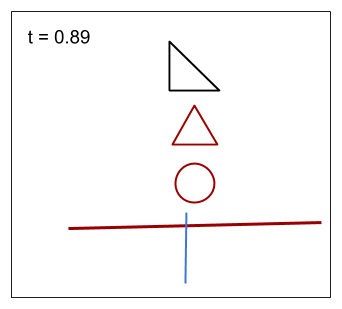
\includegraphics[keepaspectratio=true, width=0.8\textwidth]{ModeleDeNotation/i/readingTheScore.png}
\end{minipage}%
\begin{minipage}{0.45\textwidth}
\begin{lstlisting}[language = {C++}, numbers=none]
/staff/myStaff/voice/0/circle/1/name "myCircle"
/staff/myStaff/voice/0/circle/1/type "circle"
/staff/myStaff/voice/0/circle/1/x	40.6
[...]
/staff/myStaff/voice/1/triangle/1/name "myTriangle"
/staff/myStaff/voice/1/triangle/1/type "triangle"
/staff/myStaff/voice/1/triangle/1/x	40.5 
[...]
\end{lstlisting}
\end{minipage}%

\caption{Lecture temporelle d'une partition symbolist}
\label{fig:readingTheScore}
\small
\it
A gauche, une partition \emph{symbolist} entrain d'être lue: en bleu, la barre de lecture; en rouge, un staff avec deux symboles associés; en noir, un symbole libre. A droite, les informations envoyées en sortie par \emph{symbolist}, résultat de la lecture de la partition.
\end{figure}

La barre de lecture se déplace le long des symboles référents de chaque \textit{staff}. A chaque fois qu'elle rencontre un symbole associé au \textit{staff} courant, les informations du bundle OSC décrivant le symbole rencontré sont envoyées sur la sortie. Dans la figure \ref{fig:readingTheScore}, la barre de lecture a rencontrée deux symboles associés au \textit{staff} courant, leurs informations sont envoyées en sortie selon le formalisme suivant:
\begin{center}
\tiny 
/staff/<nom du staff>/voice/<numéro de la voix>/<id du symbole>/<nom d'attribut> <valeur de l'attribut>
\end{center}

Si les symboles associés à un même \textit{staff} se chevauchent, alors chaque symbole est considéré comme appartenant à une voix différente, se concrétisant par l'affichage d'un identifiant de voix différent dans les informations envoyées sur la sortie. La figure \ref{fig:readingTheScore} montre également qu'aucune information concernant le symbole libre n'est affichée. Aussi, la structure de \textit{staff} permet de séparer dans un partition les parties destinées à l'humain de celles destinées aux processus informatiques, recevant les bundles OSC.

A chaque nouveau \textit{staff} créé dans la partition, l'intervalle de temps est continué. La figure \ref{fig:stavesCreation} explicite le phénomène d'extension de l'intervalle temporel avec la création de nouveaux \textit{staff}.

\begin{figure}[H]
	\centering
	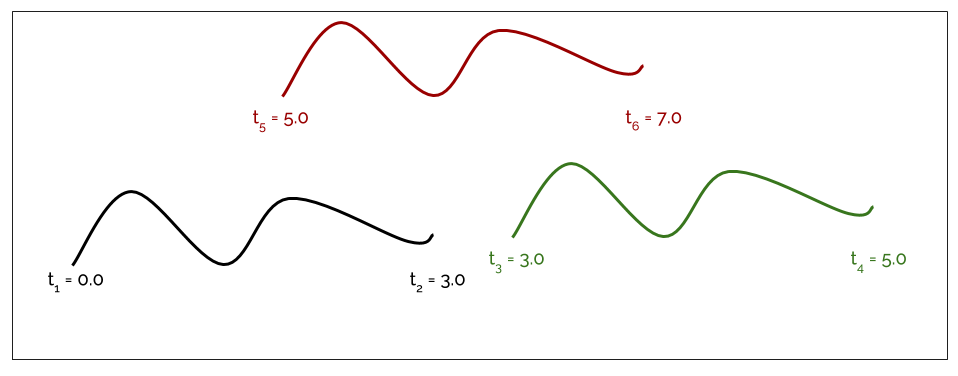
\includegraphics[keepaspectratio=true, width=0.9\textwidth]{ModeleDeNotation/i/stavesCreation.png}
	\caption{Extension de l'intervalle temporel de la partition}
	\label{fig:stavesCreation}
	\small
	\it
	En noir, le premier \emph{staff} créé définit un intervalle $[t_1, t_2]$ avec $t_1 = 0.0$ et $t_2 = 3.0$. En vert, le deuxième \emph{staff} créé définit un intervalle $[t_3, t_4]$ avec $t_3 = 3.0$ et $t_4 = 5.0$. En rouge, le troisième \emph{staff} créé définit un intervalle $[t_5, t_6]$ avec $t_5 = 5.0$ et $t_6 = 7.0$.
\end{figure}

Le placement des symboles référents de chaque \textit{staff} sur l'axe horizontal n'a pas d'incidence sur l'intervalle temporel définit; seul l'ordre de création compte. Aussi, dans la figure \ref{fig:stavesCreation}, le \textit{staff} rouge est placé avant le \textit{staff} vert sur l'axe horizontal, néanmoins il représente un intervalle temporel supérieur. 

\subsection{Concept de clef}
\label{subsec:conceptDeClef}
De fait, après avoir défini la sémantique du placement des symboles sur l'axe horizontal, la recherche de nouvelles fonctionnalités pour \textit{symbolist} a conduit à une réflexion sur la définition de la sémantique de l'axe vertical.
La CWMN (Common Western Music Notation) possède le concept de \textit{clef}, qui est un symbole placé au début d'une portée, associant à chaque ligne de la portée une hauteur représentée par un nom de note\footnote{Dans la CWMN, la hauteur d'un son est défini par un nom de note et un numéro. Par exemple, un son de fréquence 440Hz correspond au couple nom-numéro $(la, 3)$. Néanmoins, par convention, le numéro des notes est omis lors de la lecture d'une partition.}.
Aussi, les notes portent le nom de la ligne sur laquelle elles se trouvent.
La figure montre un exemple de changement de clef sur une même portée qui a pour conséquence de changer le nom des notes placées à la suite.
\begin{figure}[H]
	\centering
	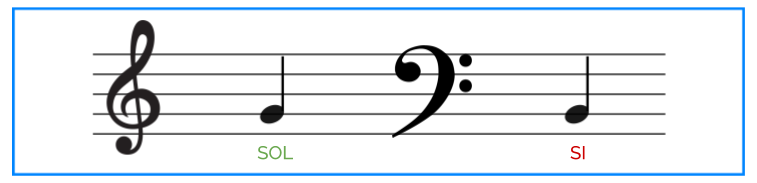
\includegraphics[keepaspectratio=true, width=0.6\textwidth]{ModeleDeNotation/i/clefsCWMN.png}
	\caption{Conséquence du changement de clefs sur le nom des notes}
	\label{fig:clefsCWMN}
	\small
	\textit{A gauche, le symbole de la clef de sol suivi d'une note placée sur la deuxième ligne de la portée. A droite, le symbole de la clef de fa suivi d'une note placée sur la deuxième ligne de la portée.}
\end{figure}
Si une clef de sol est inscrite sur la portée alors toutes les notes se trouvant à la suite sur la deuxième ligne de la portée auront pour nom \textit{sol}. Si une clef de fa est inscrite sur la portée alors toutes les notes se trouvant à la suite sur la deuxième ligne de la portée auront pour nom \textit{si}.

En s'inspirant de la CWMN, le concept de clef a été défini pour l'application \textit{symbolist}, bien qu'il ne soit pas à ce jour implémenté. Comme pour la CWMN, une clef est associé à un \textit{staff} dans \textit{symbolist}. En tirant profit du langage \textit{o.expr} (voir section \ref{subsec:odotLibrary}), une clef est définie dans \textit{symbolist} comme une liste d'expressions \textit{odot} s'appliquant à l'ensemble des symboles associés à un \textit{staff}.
 Par exemple, une clef peut déterminer l'ordre vertical des symboles attachés à un \textit{staff} comme étant la fonction inverse du message \textit{/pitch}. Dans ce cas, la clef contiendra l'expression  /y $= 1 /$ /pitch.

Pour expliciter la transformation des symboles associés à un \textit{staff} par application d'une clef, la procédure \ref{alg:applyKey} est présentée.

\begin{procedure}[H]
	\caption{ApplyKey($staff$, $clef$)}
	\label{alg:applyKey}
    
    \SetKwFunction{applyExpr}{ApplyExpr}
    
     
	\KwData{$staff$ une liste de symboles, représentant l'ensemble des symboles attachés au staff pour lequel la clef va être appliquée.}
	\KwData{$clef$ liste d'expressions \textit{odot}}
    \KwResult{L'ensemble des expressions \textit{odot} contenues dans la clef sont appliquées aux symboles du $staff$}
	
    \DontPrintSemicolon
    \BlankLine
    
	\ForEach {$expr$ t.q $expr \in clef$}{
    	\ForEach {$symbol$ t.q $symbol \in staff$}{
    		\applyExpr{$expr$, $symbol$}\;
    	}
    }    
	
\end{procedure}


\subsection{Intégration des symboles de la CWMN}
\label{integrationCWMN}
L'intégration des symboles de la CWMN est une des contributions de ce stage à l'application \textit{symbolist}.
Une analyse des besoins des compositeurs en terme d'outils de notation musicale a été menée et est présentée en annexe \ref{sec:analyseBesoins} page~\pageref{sec:analyseBesoins}. Cette analyse se présente sous la forme d'un questionnaire sur les pratiques de notation des compositeurs. A la question \og Pouvez-vous décrire votre worflow de notation? \fg, la quasi-majorité des compositeurs ont dit utiliser les outils de notation orientés CWMN dans leur phase de travail. Ce constat a donc motivé la volonté d'intégration de la CWMN dans la palette de symboles de l'application \textit{symbolist}.

Les logiciels performants pour l'édition de partitions en CWMN sont nombreux. symbolist ne prétend pas les concurrencer. De plus, les règles de mise en page d'une partition en CWMN sont pléthore et complexes. Par exemple, les techniques pour la justification horizontale des notes sur une portée est un sujet très discuté \cite{blostein1991}. Aussi, pour rester dans la philosophie de \textit{symbolist} qui est celle du dessin libre, les symboles de la CWMN ont été simplement mis à disposition dans la palette. Par la suite, l'implémentation des règles de mise en page de la notation traditionnelle sera à considérer.

Il existe une forte corrélation entre l'écriture textuelle et l'écriture musicale. Aussi, de multiple polices de caractères existent pour le texte, et il en est de même pour les polices de caractères musicaux.
Pour implanter les symboles de la CWMN dans \textit{symbolist}, la police de caractères \textit{open source} SMuFL (\textit{Standard Music Font Layout}) \cite{smufl2016}. Plus précisément, SMuFL est une spécification pour la création d'une police de caractères musicaux, maintenant soutenue par le groupe W3C Music Notation Community Group. SMuFL définit un dictionnaire de symboles musicaux (appelés des glyphes pour une police de caractères) chacun identifié par un numéro de caractère Unicode. SMuFL définit également les règles régissant la forme, la taille et la composition des caractères musicaux, et met à disposition de l'utilisateur l'ensemble de ces métadonnées dans des fichiers au format JSON.

La police de caractères \textit{Bravura}, qui est une implémentation de SMuFL, a été utilisée pour \textit{symbolist}. \textit{Bravura} est la police de caractères intégrée au logiciel de notation \textit{Dorico} développé par l'entreprise \textit{Steinberg}.
La figure donne un exemple de composition effectuée dans \textit{symbolist}, où les symboles de la police \textit{Bravura} sont mis à profit.

\begin{figure}[H]
	\centering
	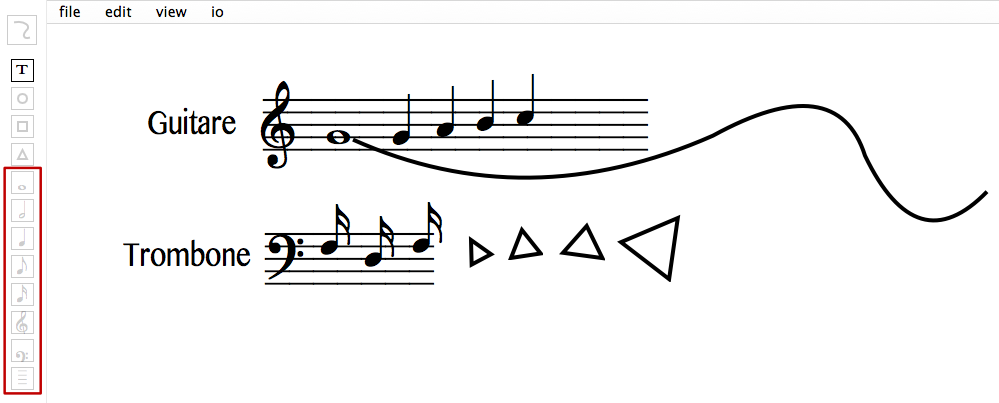
\includegraphics[keepaspectratio=true, width=\textwidth]{ModeleDeNotation/i/bravuraCreation.png}
	\caption{Composition graphique avec les caractères de la police Bravura}
	\label{fig:bravuraCreation}
	\small
	\it
	En \textcolor{red}{rouge}, quelques glyphes de la police \emph{Bravura} ajoutés à la palette de \emph{symbolist}.
\end{figure}
     